\chapter[Topic Definition]{Topic Definition}
\label{Chap:label}	%CREATE YOUR OWN LABEL.
\pagestyle{headings}


\section{Topic}

While there is no single solution that will fully protect an edge network, a common and effective way to reduce the unauthorised/unwanted network 
traffic is by simply filtering out the potentially malicious packets. While this may seem overly complex, in reality a few simple rules can be followed
to decide on whether to forward or deny/drop/block packets from entering or exiting a network. These packet filters (pf) are a type of firewall that do 
not follow any complex rules and keep state between packets or use deep packet inspection to check the contents of the payload to ensure it's not 
malicious. 

The proposed project consists of making a hardware implementation of a pf with custom Ethernet Media Access Controllers (MAC) connected to a hardware
based filtering block which is all controlled by a RISC-V softcore processor. This will then also have a web interface so that a user can configure
the rules for the pf.

\section{System Overview}


\begin{figure}[h]
    \centering
    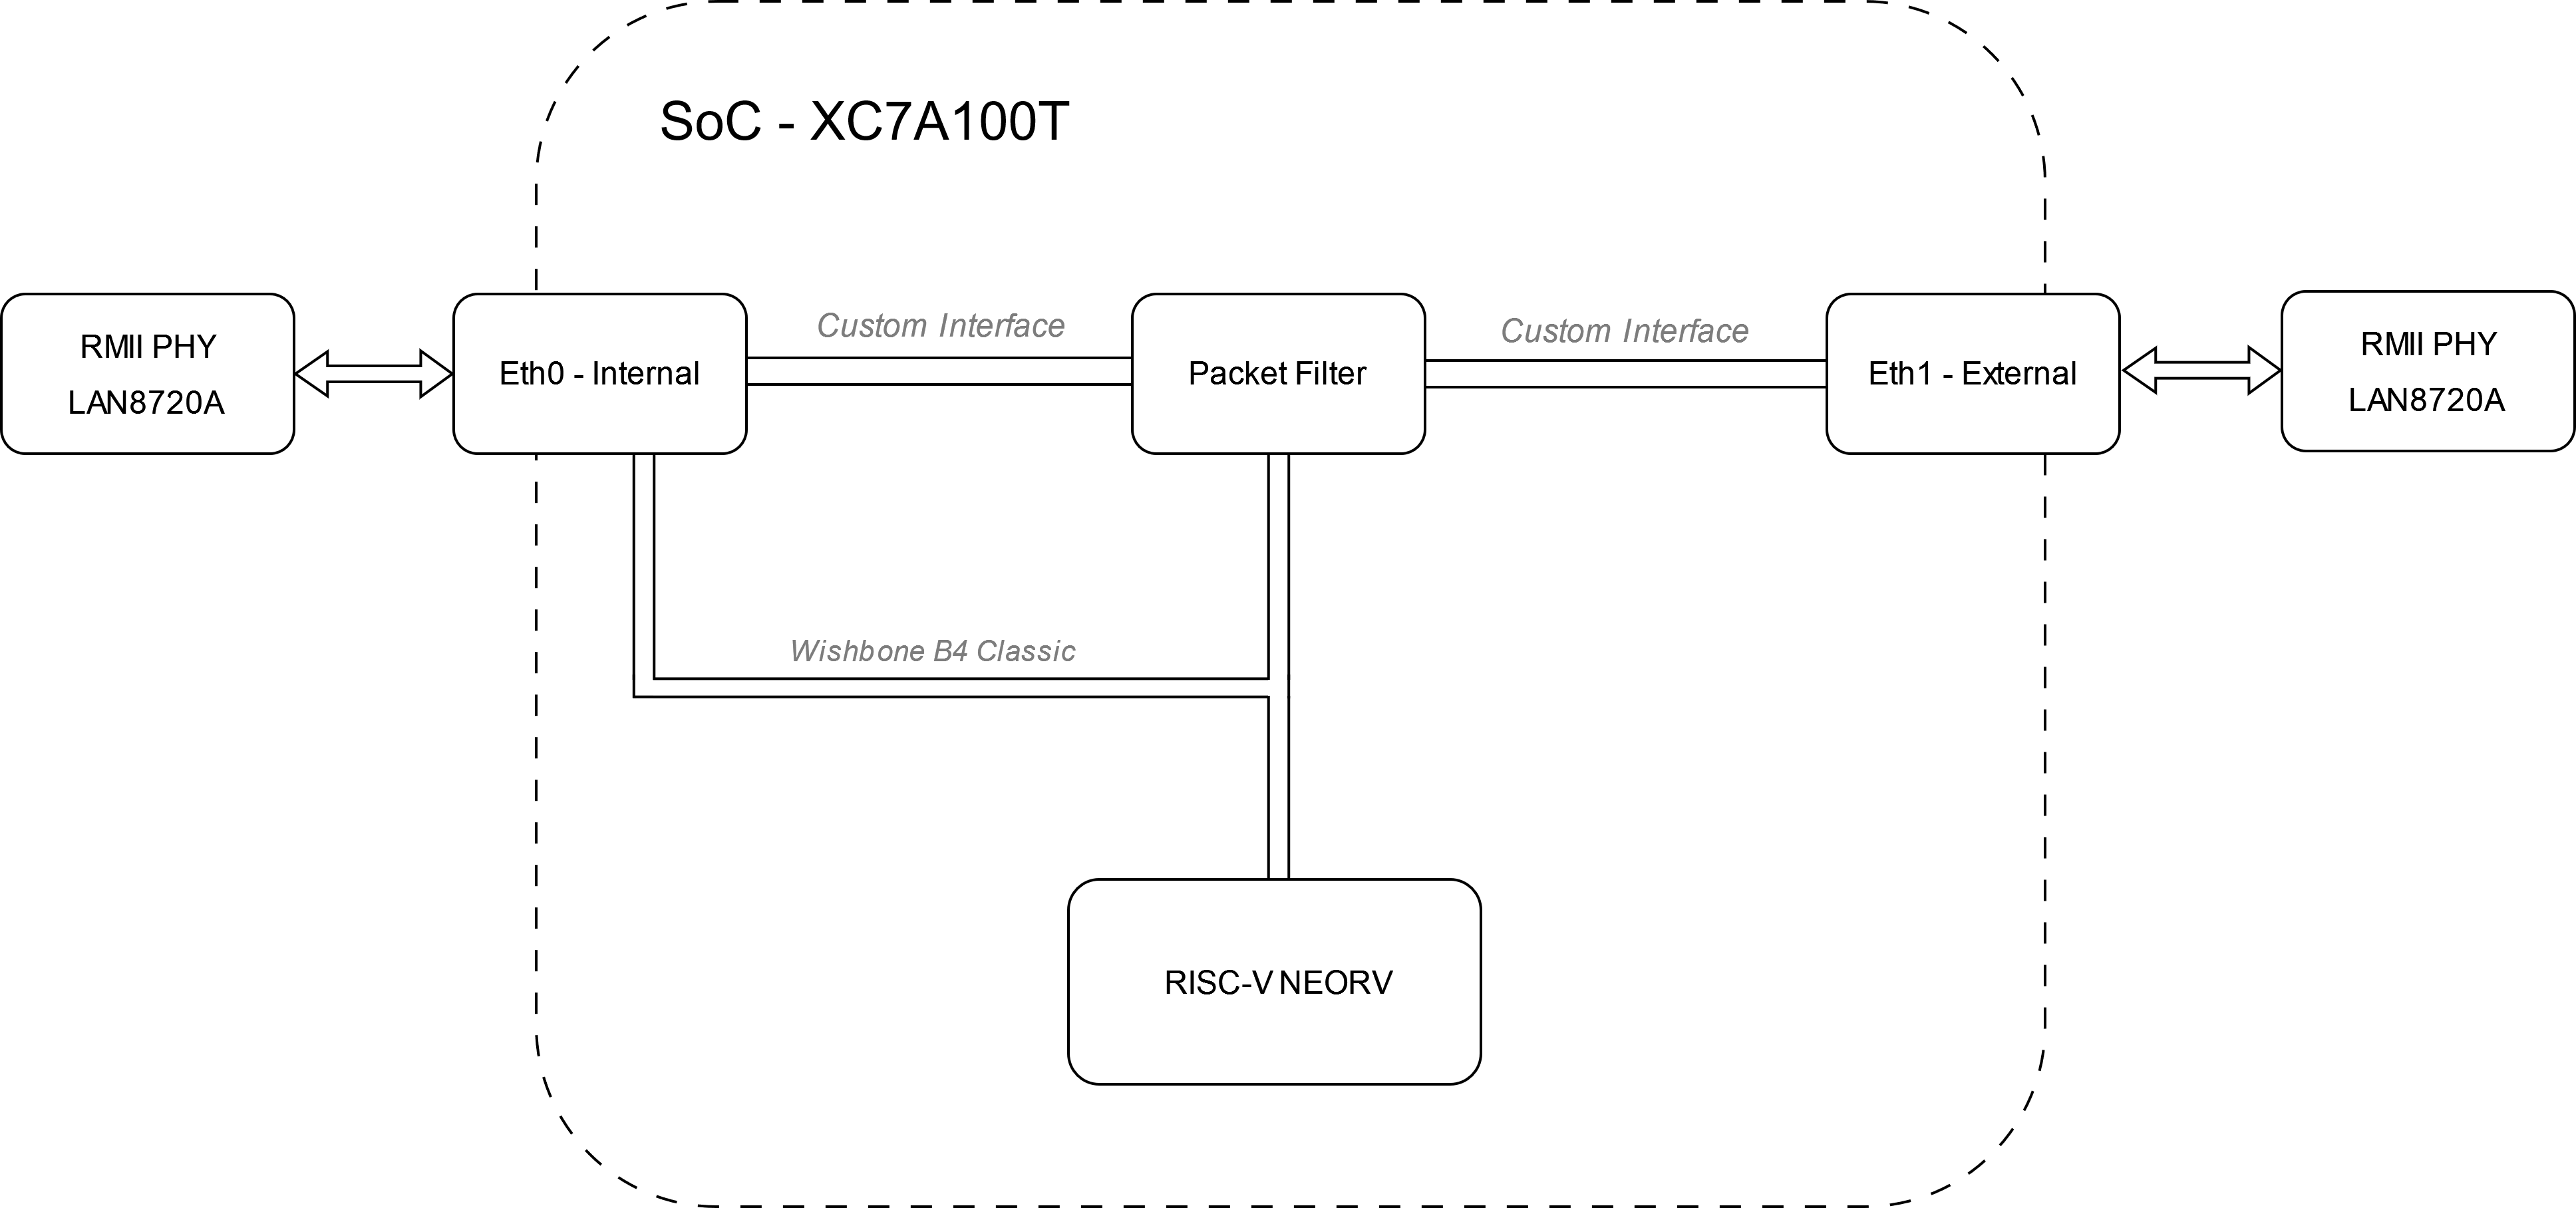
\includegraphics[width=1\textwidth]{Images/ThesisSystemsOverview.png}
    \caption{System overview}
    \label{fig:sys-overview}
\end{figure}




\section{Aims}

The aims of the proposed FPGA Ethernet controller and web interface on a RISC-V processor are:

\begin{itemize}
    \item Increase security to edge IoT networks,
    \item Increase the power efficiency for wire-speed firewalls, and
    \item Decrease the latency for packet filter firewalls.
\end{itemize}



\section{Establishing Exclusions}

While the proposed project will reduce the likelihood of network based attacks it is not a \textit{'one size fits all'} solution. 
By the nature of the IoT and edge network ecosystem, there are a myriad of different attack vectors where not all of them will be detectable at the
network level.

The proposed project will \textbf{not}
\begin{itemize}
    \item Protect against all attacks,
    \item Be able to protect against all IoT devices,
    \item Perform routing,
    \item IPv6 Packets, or
    \item Perform network address translation (NAT)
\end{itemize}



\section{Performance Indicators}



\section{Required Equiptment}
While the hardware design will be developed in such a way that it is vendor agnostic, to test the design a Digilent Nexys A7-100T developement board will be used.
Importantly, this board has a RJ45 connector and LAN8720 RMII interface chip which allows for a regular fast ethernet connection to be directly connected 
to the FPGA board. An additional LAN8720 ETH board from Waveshare is also required to obtain the secondary interface. 

To validate the functionality and effectiveness of the design, it will be compared with a Raspberry Pi Compute Module 4 (CM4) with a Waveshare CM4-DUAL-ETH-MINI 
daughterboard which contains two 1GbE interfaces. This will act as a baseline. 

\section{Technology Readiness Level}

One method for estimating the degree of maturity for a technical project is by using the \textit{Technology Readiness Levels (TRL)} benchmark. Within this, 
there are 9 levels each indicating a different phases of a design. This project is intended to reach a TRL of 6. These six different levels and their 
relevance to this project are as follows. 

\begin{enumerate}
    \item \textbf{TRL 1: Basic Research} - The concepts are researched and a base understanding of the system is gathered,
    \item \textbf{TRL 2: Applied Research} - Detailed research is conducted into each part of the project,
    \item \textbf{TRL 3: Proof of Concept} - A cutdown version of the final project protoype that highlights the core functionality or subsystems working,
    \item \textbf{TRL 4: Lab Testing of Prototype} - Prototype of the core design with majority of the functionality working,
    \item \textbf{TRL 5: Testing of Integrated system} - Refined prototype that works as intended but may be incomplete, and
    \item \textbf{TRL 6: Prototype System Verified} - Comparison to pre-existing solutions and verification. 
\end{enumerate}


